\documentclass[12pt]{article}

\usepackage{fullpage}
\usepackage{mdframed}
\usepackage{colonequals}
\usepackage{algpseudocode}
\usepackage{algorithm}
\usepackage{tcolorbox}
\usepackage[all]{xy}
\usepackage{proof}
\usepackage{mathtools}
\usepackage{bbm}
\usepackage{amssymb}
\usepackage{amsthm}
\usepackage{amsmath}
\usepackage{amsxtra}
\newcommand{\bb}{\mathbb}


\newtheorem{theorem}{Theorem}[section]
\newtheorem{corollary}{Corollary}[theorem]
\newtheorem{lemma}{Lemma}

\newcommand{\mathcat}[1]{\textup{\textbf{\textsf{#1}}}} % for defined terms

\newenvironment{problem}[1]
{\begin{tcolorbox}\noindent\textbf{Problem #1}.}
{\vskip 6pt \end{tcolorbox}}

\newenvironment{enumalph}
{\begin{enumerate}\renewcommand{\labelenumi}{\textnormal{(\alph{enumi})}}}
{\end{enumerate}}

\newenvironment{enumroman}
{\begin{enumerate}\renewcommand{\labelenumi}{\textnormal{(\roman{enumi})}}}
{\end{enumerate}}

\newcommand{\defi}[1]{\textsf{#1}} % for defined terms

\theoremstyle{remark}
\newtheorem*{solution}{Solution}

\setlength{\hfuzz}{4pt}

\newcommand{\calC}{\mathcal{C}}
\newcommand{\calF}{\mathcal{F}}
\newcommand{\C}{\mathbb C}
\newcommand{\N}{\mathbb N}
\newcommand{\Q}{\mathbb Q}
\newcommand{\R}{\mathbb R}
\newcommand{\Z}{\mathbb Z}
\newcommand{\br}{\mathbf{r}}
\newcommand{\RP}{\mathbb{RP}}
\newcommand{\CP}{\mathbb{CP}}
\newcommand{\nbit}[1]{\{0, 1\}^{#1}}
\newcommand{\bits}{\{0, 1\}^{n}}
\newcommand{\bbni}{\bigbreak \noindent}
\newcommand{\norm}[1]{\left\vert\left\vert#1\right\vert\right\vert}

\let\1\relax
\newcommand{\1}{\mathbf{1}}
\newcommand{\fr}[2]{\left(\frac{#1}{#2}\right)}

\newcommand{\vecz}{\mathbf{z}}
\newcommand{\vecr}{\mathbf{r}}
\DeclareMathOperator{\Cinf}{C^{\infty}}
\DeclareMathOperator{\Id}{Id}

\DeclareMathOperator{\Alt}{Alt}
\DeclareMathOperator{\ann}{ann}
\DeclareMathOperator{\codim}{codim}
\DeclareMathOperator{\End}{End}
\DeclareMathOperator{\Hom}{Hom}
\DeclareMathOperator{\id}{id}
\DeclareMathOperator{\M}{M}
\DeclareMathOperator{\Mat}{Mat}
\DeclareMathOperator{\Ob}{Ob}
\DeclareMathOperator{\opchar}{char}
\DeclareMathOperator{\opspan}{span}
\DeclareMathOperator{\rk}{rk}
\DeclareMathOperator{\sgn}{sgn}
\DeclareMathOperator{\Sym}{Sym}
\DeclareMathOperator{\tr}{tr}
\DeclareMathOperator{\img}{img}
\DeclareMathOperator{\CandE}{CandE}
\DeclareMathOperator{\CandO}{CandO}
\DeclareMathOperator{\argmax}{argmax}
\DeclareMathOperator{\first}{first}
\DeclareMathOperator{\last}{last}
\DeclareMathOperator{\cost}{cost}
\DeclareMathOperator{\dist}{dist}
\DeclareMathOperator{\path}{path}
\DeclareMathOperator{\parent}{parent}
\DeclareMathOperator{\argmin}{argmin}
\DeclareMathOperator{\excess}{excess}
\let\Pr\relax
\DeclareMathOperator{\Pr}{\mathbf{Pr}}
\DeclareMathOperator{\Exp}{\mathbb{E}}
\DeclareMathOperator{\Var}{\mathbf{Var}}
\let\limsup\relax
\DeclareMathOperator{\limsup}{limsup}
%Paired Delims
\DeclarePairedDelimiter\ceil{\lceil}{\rceil}
\DeclarePairedDelimiter\floor{\lfloor}{ \rfloor}


\newcommand{\dagstar}{*}

\newcommand{\tbigwedge}{{\textstyle{\bigwedge}}}
\setlength{\parindent}{0pt}
\setlength{\parskip}{5pt}


\begin{document}

\title{CS 40: Computational Complexity}

\author{Sair Shaikh}
\maketitle

% Collaboration Notice: Talked to Henry Scheible '26 to discuss ideas.


\begin{problem}{1}
    (1.3.18) For a path-connected, locally path-connected, and semilocally simply connected space $X$, call a path-connected covering $p \colon E \to X$ \emph{abelian} if it is normal and has abelian deck transformation group. Show that $X$ has an abelian covering space that is a covering space of every other abelian covering space of $X$ and that such a `universal' abelian covering space is unique up to equivalence. Describe this covering space explicitly for $X = S^1 \vee S^1$ and $S^1 \vee S^1 \vee S^1$. 
\end{problem}

\begin{solution}
    Since $X$ is path-connected, locally path-connected, and semilocally simply connected, we note that it it has a universal cover $\tilde\rho: \tilde{B} \to X$. Let $H \subseteq G := \pi_1(X, x_0)$ be the commutator (i.e. generated by elements $[g, h]$ for $g, h \in G$). By the existence of covers theorem, there exists a covering space $\rho: (E, e_0) \to (X, x_0)$ such that $\rho_*(\pi_1(E, e_0)) = H$. We claim that $(E, \rho)$ is the unique universal abelian covering space of $X$. \bbni
    Note that since $H$ is the commutator subgroup, it is normal. To see this, let $[a,b] \in H$ be a generator, and $g \in G$. Then, 
    \begin{align*}
        g[a,b]g^{-1} &= ga^{-1}b^{-1}abg^{-1} \\
        &= ga^{-1}(g^{-1}g)b^{-1}(g^{-1}g)a(g^{-1}g)bg^{-1} \\
        &= (ga^{-1}g^{-1})(gb^{-1}g^{-1})(gag^{-1})(gbg^{-1}) \\
        &= (gag^{-1})^{-1}(gbg^{-1})^{-1}(gag^{-1})(gbg^{-1}) \\
        &= [gag^{-1}, gbg^{-1}] \in H
    \end{align*}
    Thus, $H$ is normal in $G$ and $(E, \rho)$ is a normal covering space. \bbni
    Moreover, by the normal covering theorem, we know that the deck transformation group is equal to $G/H$. However, since $H$ is the commutator, we have that $G/H$ is abelian (by definition of the commutator). Thus, $(E, \rho)$ is an abelian covering space. \bbni
    Moreover, if $(E', \rho')$ was another normal cover corresponding to $H' \subseteq G$ with abelian deck transformation group $G/H'$, then since $G/H'$ is abelian, we must have that $H \subseteq H'$ (the commutator must be quotiented out for the result to be abelian). Thus, we have that:
    \[ \rho_*(\pi_1(E, e_0)) \subseteq \rho_*'(\pi_1(E', e_0'))\]
    Since $E$ is path-connected and locally path-connected (as it is a cover of locally path-connected $X$), we can apply the general lifting theorem to get a map $f: (E, e_0) \to (E', e_0')$ such that:
    \[ \rho' \circ f = \rho \]
    By functoriality, we have that:
    \[ \rho'_* \circ f_* = \rho_* \]
    Since $\rho_*$ is injective, we have that $f_*$ is injective. Thus, 
    \[ f_*(\pi_1(E, e_0)) \subseteq \pi_1(E', e_0')\]
    is a subgroup. Thus, by the Galois correspondence, we have that $f: (E, e_0) \to (E', e_0')$ is a covering map. \bbni 
    Uniqueness follows directly from the universal property. If $A, B$ are two universal abelian covers, then by the universal property, there exists unique covering maps $f: A \to B$ and $g: B \to A$ that commute with the covering maps of $A$ and $B$. However, then $g \circ f$ is a covering map from $A$ to itself. By the uniqueness of lifts, we must have $g \circ f = \id_A$. Similarly, we have that $f \circ g = \id_B$. Thus, $f$ and $g$ are homeomorphisms, and the universal abelian cover is unique up to equivalence. \bbni 
    For $X = S^1 \vee S^1$, we have that $\pi_1(S^1 \vee S^1) = \Z * \Z$. Let $H$ be the commutator subgroup of $\Z * \Z$. We want a cover of $S^1 \vee S^1$ corresponding the commutator subgroup. \\
    Let $E \subset \R^2$ be the $1$-skeleton of the 2d integer lattice, and $\rho: (E, e_0) \to (S^1 \vee S^2 )$ map an integer interval $(n, n+1) \times \{m\}$ to the first circle, and $\{m\} \times (n, n+1)$ to the second circle (this is a cover as each interval maps homeomorphically onto a circle) and all vertices map to the wedge point. Then, the deck transformation group of $E$ is $\Z^2$ by translation. Note that this acts transitively on the fiber over the wedge point (the lattice $\Z^2$), thus the cover is normal. Thus, by the the normal covering theorem, we have that:
     \[ \text{Deck}(E) = \Z^2 = \pi_1(S^1 \vee S^1)/\rho_*(\pi_1(E, e_0)) \]
     Thus, we have $\rho_*(\pi_1(E, e_0)) = H$ and by uniqueness (the Galois correspondence), we have that $E$ is the unique universal abelian cover of $S^1 \vee S^1$. \bbni
     Similarly, for $X = S^1 \vee S^1 \vee S^1$, we let $E \subset \R^3$ the $1$-skeleton of the 3d integer lattice. We can map the integer intervals of the lattice in each dimension to the first, second, and third circles respectively. Then, the deck transformation group of $E$ is $\Z^3$ by translation. Note that this acts transitively on the fiber over the wedge point (the lattice $\Z^3$), thus the cover is normal. Thus, by the the normal covering theorem, we have that: 
    \[ \text{Deck}(E) = \Z^3 = \pi_1(S^1 \vee S^1 \vee S^1)/\rho_*(\pi_1(E, e_0)) \]
    Thus, we have $\rho_*(\pi_1(E, e_0)) = H$, the commutator subgroup, and by uniqueness (the Galois correspondence), we have that $E$ is the unique universal abelian cover of $S^1 \vee S^1 \vee S^1$.
\end{solution}
\newpage

\begin{problem}{2}
    (1.3.20) Construct non-normal covering spaces of a Klein bottle by a Klein bottle and by a torus. 
\end{problem}

\begin{solution}
    \bbni
    \begin{center}
        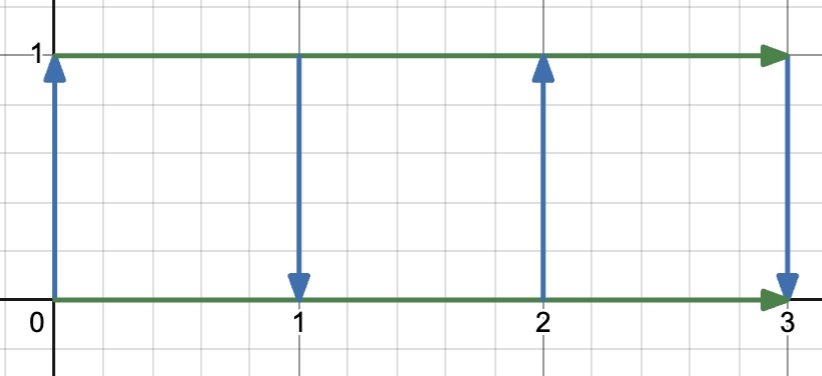
\includegraphics{hwk6_kleincover.png}
    \end{center}
    Consider the given $3$-sheeted cover of the Klein bottle by a Klein bottle. Each of the squares in the cover is a copy of the Klein bottle, which the whole rectangle is also a Klein bottle. Consider the loop that is the image of the loop $a$ marked by the leftmost edge of the cover (the two endpoints are identified). This maps to a loop based at the image of the point $(0, 0)$ in the Klein bottle. However, considering the lift of this loop to the middle sheet, we note that the lift of this loop is not a loop, as the two endpoints of the 2nd left-most blue edge are not identified. Thus, the deck transformation group is not transitive and the cover is not normal. \bbni
    \begin{center}
        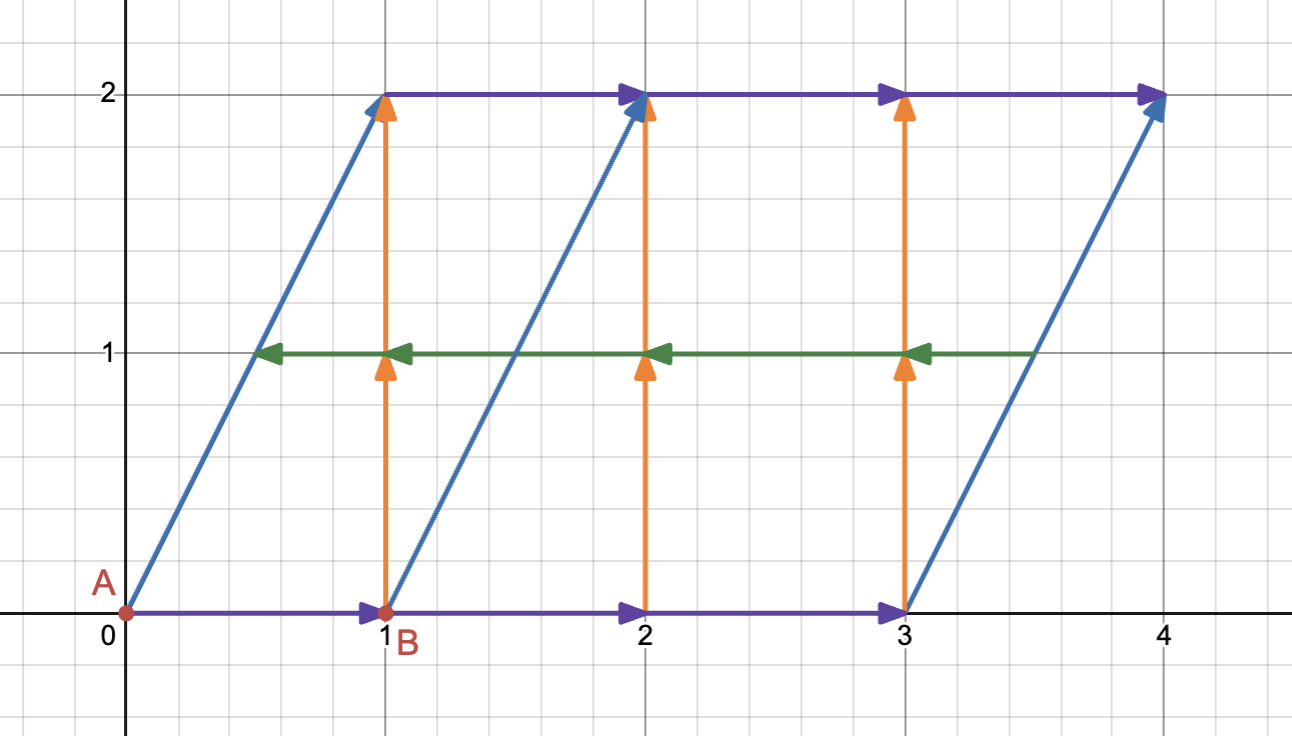
\includegraphics[width=0.8\textwidth]{hwk6_toruscover.png}
    \end{center}
    Consider the following $6$-sheeted cover of the torus by a Klein bottle. Note that each square in the cover is a copy of the Klein bottle, and the whole rectangle is a torus. Consider the loop in the cover marked by the leftmost blue edge. The image of this loop in the torus is a loop based at the image of the point $A$. However, considering the lift of this point starting at $B$, we note that the two endpoints of this path are not identified in the cover, thus it is not a loop. Thus, the deck transformation group is not transitive and the cover is not normal.
\end{solution}
\newpage

\begin{problem}{3}
    (1.3.29) Let $Y$ be path-connected, locally path-connected, and simply connected. Let $G_1$ and $G_2$ be two subgroups of $\mathrm{Homeo}(Y)$ defining covering space actions on $Y$. Show that the orbit spaces $Y/G_1$ and $Y/G_2$ are homeomorphic if and only if $G_1$ and $G_2$ are conjugate subgroups of $\mathrm{Homeo}(Y)$. 
\end{problem}

\begin{solution}
    Let $G_1$ and $G_2$ be two conjugate subgroups of $\mathrm{Homeo}(Y)$. Then, there exists an homeomorphism $\phi: Y \to Y$ such that: $\phi G_1 = G_2\phi$. For all $x \in Y$:
    \begin{align*}
        \phi(G_1 x) &= \phi G_1 \cdot x \\ 
        &= G_2 \phi \cdot x \\
        &= G_2 \cdot \phi(x)
    \end{align*} 
    Thus, the map $\tilde\phi: Y/G_1 \to Y/G_2$, taking $[G_1 x] \mapsto [G_2 \phi(x)]$ is well-defined. Moreover, if $q_1: Y \to Y/G_1$ and $q_2: Y \to Y/G_2$ are the quotient maps, then:
    \[ \tilde \phi \circ q_1 = q_2 \circ \phi\]
    Thus, $\tilde \phi$ is continous, as the RHS is continous and $q_1$ is open and surjective (if $U \subseteq Y/G_2$ is open, then, $\phi^{-1} \circ q_2^{-1}(U)$ is open in $Y$. Moreover, as $q_1$ is open and surjective, we have that $q_1$ of this is open and equal to $\tilde\phi^{-1}(U)$). \bbni
    Next, since $\phi^{-1}G_2 = G_1\phi^{-1}$, we similarly get $\phi^{-1}$ continous mapping $[G_2 x] \mapsto [G_1 \phi^{-1}(x)]$. As $\phi$ and $\phi^{-1}$ are inverses, clearly $\tilde \phi$ and $\tilde \phi^{-1}$ are inverses. Thus, $Y/G_1$ and $Y/G_2$ are homeomorphic. \bbni
    Now assume $f: Y/G_1 \to Y/G_2$ is a homeomorphism. Note that since $G_1$ and $G_2$ define covering space actions on $Y$, we have the normal covers $\rho_1: Y \to Y/G_1$ and $\rho_2: Y \to Y/G_2$. Then, we have that: 
    \[ f \circ \rho_1: Y \to Y/G_2\]
    is also a cover as $f$ is a homeomorphism. Since $Y$ is simply connected, and hence a universal cover, the push-forwards of $\pi_1(Y)$ are trivial, hence equal, thus the covers are equivalent. Thus, there exists a lift to a deck transformation $\tilde f \in \mathrm{Homeo}(Y)$ such that: 
    \[ f \circ \rho_1 = \rho_2 \circ \tilde f\]
    Thus, for $g_1 \in G_1$, we have that: 
    \[\rho_1  \circ g_1 = \rho_1\]
    as applying $g_1$ stays in the same $G_1$ orbit. Thus, we have that: 
    \begin{align*}
        \rho_2 \circ \tilde f \circ g_1 &= f \circ \rho_1 \circ g_1 \\
        &= f \circ \rho_1 \\
        &= \rho_2 \circ \tilde f
    \end{align*} 
    Thus, we have: 
    \[ \rho_2 \circ (\tilde f \circ g_1 \circ \tilde f^{-1}) = \rho_2 \circ \tilde f \circ \tilde f^{-1} = \rho_2\]
    Thus, we have that $\tilde f \circ g_1 \circ \tilde f^{-1} \in G_2$. Thus, we have that: 
    \[ \tilde f G_1\tilde f^{-1} \subseteq G_2\]
    Symmetrically, arguing using $\tilde f^{-1}$, we have that: 
    \[ \tilde f^{-1} G_2\tilde f \subseteq G_1\]
    Thus, $G_1$ and $G_2$ are conjugate subgroups of $\mathrm{Homeo}(Y)$.
\end{solution}
\newpage

\begin{problem}{4}
    (2.1.10) Show that if $A$ is a retract of $X$, then the map $H_n(A) \to H_n(X)$ induced by the inclusion of $A$ in $X$ is injective for all $n$. 
\end{problem}

\begin{solution}
    Let $\iota: A \to X$ be the inclusion map and $r: X \to A$ be the retraction.     The problem is evident from noting that taking the chain homotopy and then homology are functors, thus preserve identities and compositions, and that $r \circ \iota = \id_A$. We spell this out more as follows. \bbni
    Since mapping to the chain complex is a functor, we have the maps $\iota_{*n}: C_n(A) \to C_n(X)$ and $r_{*n}: C_n(X) \to C_n(A)$ that satisfy: 
    \[  r_{*n} \circ \iota_{*n} = \id_{C_n(A)}\]
    for all $n$ (since the identity in the category of chain complexes is the identity on each element in the chain). Then, since taking the $i$th homology group is a functor, we have the maps $\iota_{**n}: H_n(A) \to H_n(X)$ and $r_{**n}: H_n(X) \to H_n(A)$ that satisfy: 
    \[ r_{**n} \circ \iota_{**n} = \id_{H_n(A)}\]
    Thus, since $\id_{H_n(A)}$ is bijective, we have that $\iota_{*n}$ is injective.
\end{solution}
\newpage

\begin{problem}{5}
    (2.1.11) Show that chain homotopy is an equivalence relation on the set of chain maps between two chain complexes.
\end{problem}

\begin{solution}
    Let $(C_n, \delta)$ and $(D_n, \delta')$ be two chain complexes. We need to show that chain homotopy is reflexive, symmetric, and transitive. We prove these indiivudally:
    \begin{itemize}
        \item[(Reflexive.)] Let $f_n: C_n \to D_n$ be a chain map. Pick $s_n: C_n \to D_n$ to be the zero map. Then, we have that: 
        \[ \delta'_{i+1} \circ s_i + s_{i-1} \circ \delta_i = 0 = f_i - f_i\]
        Thus, $s_n$ gives a chain homotopy between $f_n$ and itself. Thus, the relation is reflexive. 
        \item[(Symmetric)] Let $f_n, g_n: C_n \to D_n$ be two chain maps. Let $s_n: C_n \to D_{n+1}$ be a chain homotopy between $f_n$ and $g_n$. Then, we have that:
        \[ \delta'_{i+1} \circ s_i + s_{i-1} \circ \delta_i = f_i - g_i\]
        Since the elements in the chain complex are groups, they have inverses. Thus, we can define the maps $s_n': C_n \to D_{n+1}$ to be $-s_n$. Moreover, as all of these maps are homomorphisms, we can pull the inverse out as $\psi(-a) = -\psi(a)$ for any group homomorphism $\psi$ and element $a$. Then, we have that:
        \begin{align*}
            \delta'_{i+1} \circ s'_i + s'_{i-1} \circ \delta_i &= -\delta'_{i+1} \circ s_i - s_{i-1} \circ \delta_i\\ 
            &= -\left( \delta'_{i+1} \circ s_i + s_{i-1} \circ \delta_i \right) \\
            &= -\left( f_i - g_i \right) \\
            &= g_i - f_i
        \end{align*}
        Thus, $s_n'$ gives a chain homotopy between $g_n$ and $f_n$. Thus, the relation is symmetric.
        \item[(Transitive)] Let $f_n, g_n, h_n: C_n \to D_n$ be three chain maps. Let $s_n: C_n \to D_{n+1}$ be a chain homotopy between $f_n$ and $g_n$ and $t_n: C_n \to D_{n+1}$ be a chain homotopy between $g_n$ and $h_n$. Then, we have that:
        \begin{align*}
            \delta'_{i+1} \circ s_i + s_{i-1} \circ \delta_i &= f_i - g_i\\
            \delta'_{i+1} \circ t_i + t_{i-1} \circ \delta_i &= g_i - h_i
        \end{align*}
        Thus, we can add these two equations together and write (where the addition is point-wise in the codomain):
        \begin{align*}
            \delta'_{i+1} \circ (s_i + t_i) + (s_{i-1} + t_{i-1}) \circ \delta_i &= f_i - g_i + g_i - h_i\\
            &= f_i - h_i
        \end{align*}
        Thus, we can define the map $p_n := s_n + t_n: C_n \to D_{n+1}$. This is then a chain homotopy between $f_n$ and $h_n$. Thus, the relation is transitive.
    \end{itemize}
    Thus, we have shown that chain homotopy is reflexive, symmetric, and transitive. Thus, it is an equivalence relation on the set of chain maps between two chain complexes.
\end{solution}

\end{document}